\chapter{Multiresolution Imaging}

This chapter describes the implementation and experiments of the MR-Net for imaging applications. Imaging applications benefit greatly from multiresolution representations, as they allow us to represent an image hierarchically at different levels of details. This hierarchical model is aligned with some classical image and human visual perception models~\cite{marr82}, and it is instrumental for many tasks in computer vision and graphics, such as compression, analysis and rendering. 

For example, in image compression, we can use a multiresolution representation to identify and discard details that are not perceptually important, while preserving important features of the image. This can significantly reduce the amount of data needed to represent the image, while still maintaining its overall quality~\cite{burt1987laplacian}. Additionally, in rendering, multiresolution representations have built-in support for antialiasing, which traditionally is implemented using image pyramids~\cite{mipmap83}. Another important applications of imaging in Graphics is texture synthesis. In that realm, besides antialiasing, the creation of visual patterns from examples has great relevance~\cite{thies19}.

Traditionally, multiresolution representations for images have been based on signal processing techniques derived from Fourier theory~\cite{bracewell1986fourier}. Such operators were primarily motivated by image compression~\cite{bhaskaran1997image} and played an important role in the development of JPEG-2000~\cite{marcellin2000overview}. For instance, the Discrete Cosine Transform \cite{dct-og} have been  used as an efficient way to get a frequency content of the image, and estimate the importance of certain coefficients to the image quality perception. 

Although Fourier transforms were initially popular for decomposing signals into multiple frequencies, the wavelet transform, introduced by \citet{mallat1989theory}, soon gained popularity as it enabled representing a signal in levels of detail and scale, and was widely applied to a first generation of wavelet-based image codecs~\cite{antonini1992image}. Subsequently, wavelet analysis of multiscale edges led to a second generation of image coding methods, with higher compression rates~\cite{mallat-2gen}. Nevertheless, understanding and controlling the frequencies present in a signal has been critical on interpreting its details and avoiding artifacts such as aliasing. In this sense, sinusoidal  functions have been instrumental in the development of the multiresolution theory.


\section{Multiresolution Image Representation}
\label{s:img}


In the following experiments, we adopt the M-Net subclass of the architecture, and the level of detail scheme based on the Gaussian Pyramid in all examples. The multiresolution for the image Pyramid is according to a dyadic structure, i.e., $2^j$. The Image Pyramid is built by filtering with a Gaussian kernel and decimation.

We have designed the MR-Module considering an empirical exploration of the sub-network capacity to represent images with typical characteristics (i.e., photographs). Each stage has a width of $96$ neurons for all layers on its first, hidden, and linear blocks. In each stage, the hidden block has only a single layer.

We have determined that the base resolution of the train data at the first stage should be $2^3 = 8$, and we have chosen the number of stages of the network based on the resolution of the image to be represented. Unless otherwise indicated, the images used in the experiments have a resolution of 512, in which case the pyramid is composed of the following resolution levels: 8, 16, 32, 64, 128, 256, and 512. Consequently, the network has a total of 7 stages.

We train the network using an adaptive scheme with the following hyper-parameters: Loss Function used is MSE (Mean Squared Error); convergence threshold = $0.001$ (i.e., training of a stage stops if loss value changes less than $0.001\%$); maximum number of epochs per stage of $300$; each epoch visits all the pixels once; size of mini-batch of $65536$ (to fit the GPU memory). Training uses Adam with a learning rate of $1e-4$.

% {\color{red}}
The network initialization follows the scheme in Sec. \ref{s-frequency-initialization}, with the choice of frequency bands described in the "Filtering with Gaussian pyramid" level of detail scheme (Sec. \ref{s:lod}). The weights of first layer of each stage are set to match the frequencies of the corresponding level of detail: $\omega_0$ is uniformly distributed as $ \mathcal{U}(-B_i, B_i)$ with $B_i = [4, 8, 16, 32, 64, 128, 256]_{i=1}^7$ for a network with seven stages, and $\omega_h = 30$ for all experiments.


\subsection{Level of Detail Example}
\label{ss:LOD}

We now show an example of a multiresolution image representation using the setup described above. For this experiment, we chose the ``Cameraman'', a standard test image used in the field of image processing and also in \citet{sitzmann2019siren}.
The source is a monochromatic picture with $512\times 512$ pixels of resolution.

Fig~\ref{f:lod} depicts the levels 1, 3, 5 and 7 of the multiresolution reconstructed with resolution of $512\times 512$, as well as the corresponding Fourier spectra. 

\begin{figure}[!ht]
\centering

\includegraphics[width=0.20\linewidth]{img/ch5/1-cameraman.png}

\includegraphics[width=0.20\linewidth]{img/ch5/3-cameraman.png}
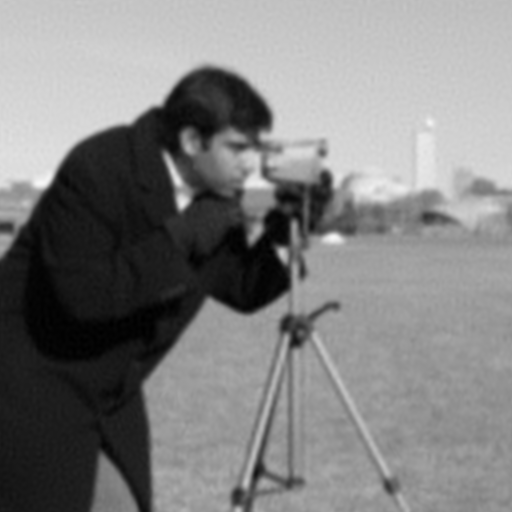
\includegraphics[width=0.20\linewidth]{img/ch5/5-cameraman.png}
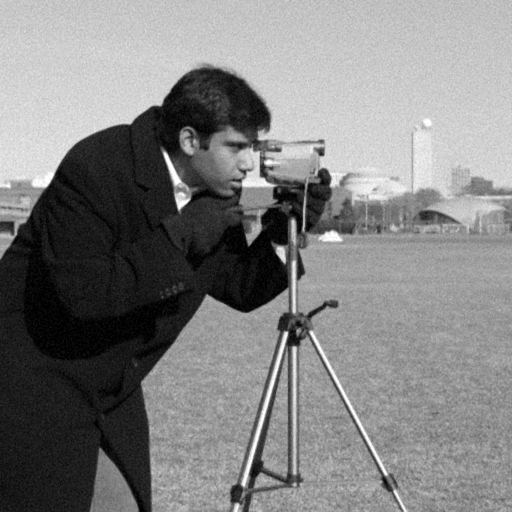
\includegraphics[width=0.20\linewidth]{img/ch5/7-cameraman.png} \\
\vspace{1pt}

\includegraphics[width=0.20\linewidth]{img/ch5/1-fft.png}
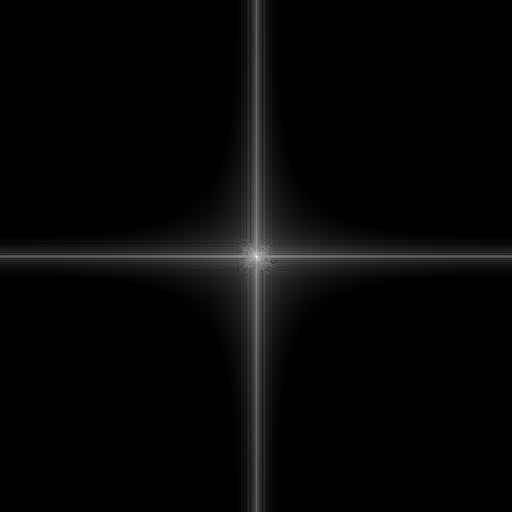
\includegraphics[width=0.20\linewidth]{img/ch5/3-fft.png}
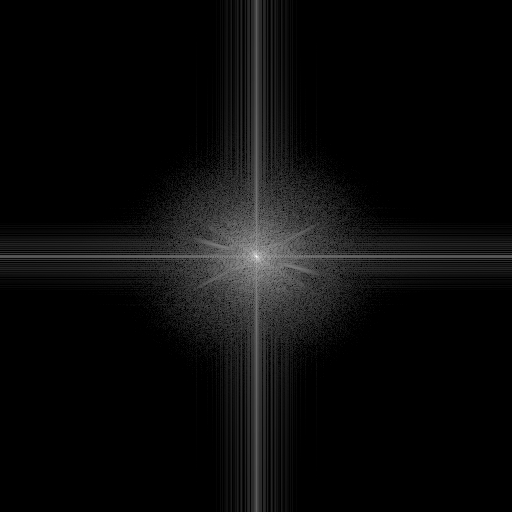
\includegraphics[width=0.20\linewidth]{img/ch5/5-fft.png}
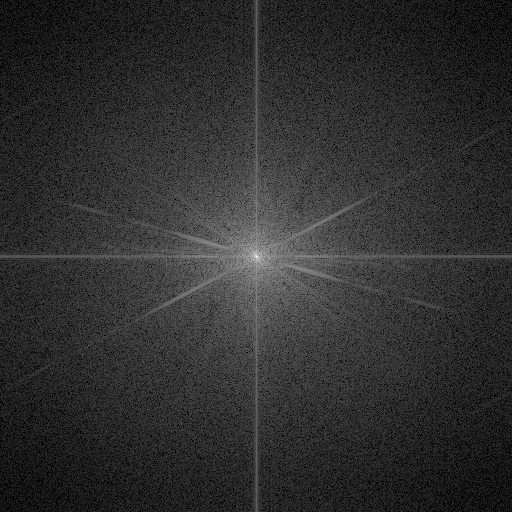
\includegraphics[width=0.20\linewidth]{img/ch5/7-fft.png}
\caption{Cameraman - reconstructed multiresolution levels 1, 3, 5 and 7 and corresponding Fourier spectra.}
\label{f:lod}
\end{figure}

The training times for each stage of the networks are as follows: 5s, 4s, 3s, 11s, 17s, 29s and 48s. The total training time is 117s. The machine was a Windows 10 laptop with a NVIDIA RTX A5000 Laptop GPU. Note that these times result from the adaptive training regime and the number of samples for each level of the Gaussian Pyramid. 

The training evolution is depicted in the graph of Fig~\ref{f:training-epochs} that shows the convergence of the MSE loss with the number of epochs for each multiresolution levels 1, 3, 5, and 7. It is worth pointing out the qualitative behavior of the network, in that the base level (stage 1) takes more than 200 epochs to reach the limit, while detail levels (stages 3, 5, 7) take less than 150 epochs to converge. Also, the error decreases for each level of detail. It is like, there are two different modes, one to fit the base level and the other for the detail levels.

\begin{figure}[!h]
\centering
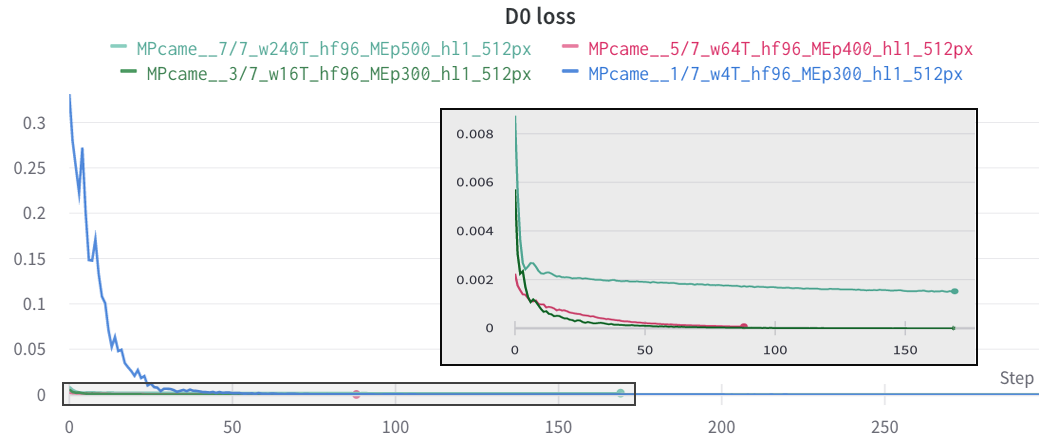
\includegraphics[width=\linewidth]{img/ch5/stages-training-epochs.png}
\caption{Qualitative convergence behavior for Cameraman in Fig~\ref{f:lod}.}
\label{f:training-epochs}
\end{figure}


The inference time for image reconstruction, varies from 0.02 seconds on the GPU to 0.7 seconds on the CPU, which is sufficiently fast for interactive visualization.

\subsection{Texture}

The second imaging example is the usage of the MR-Net representation to model texture and patterns. Arguably, visual textures constitute one of the most important applications for images in diverse fields, ranging from photo-realistic simulations to interactive games. Currently, more and more image rendering relies on some kind of graphics acceleration, sometimes through GPUs integrated with Neural Engines. In that context, it is desirable to have a neural image representation that is compact and supports the level of detail.

For the experiment shown in this subsection we have chosen an image of woven fabric background with patterns. The characteristics of this texture allows us to explore the limits of visual patterns at different resolutions. The original image has a resolution of $1025\times 1025$ pixels and the corresponding model contains 5 levels of detail.

In Fig~\ref{f:pattern} we show our experiments, where Fig.~\ref{f:pattern}(b) shows the image in the original resolution, while Fig.~\ref{f:pattern}(a) shows a zoom-in and Fig.~\ref{f:pattern}(c) shows a zoom-out.

\begin{figure}[!h]
\centering
\begin{subfigure}{0.39\linewidth}
  \centering
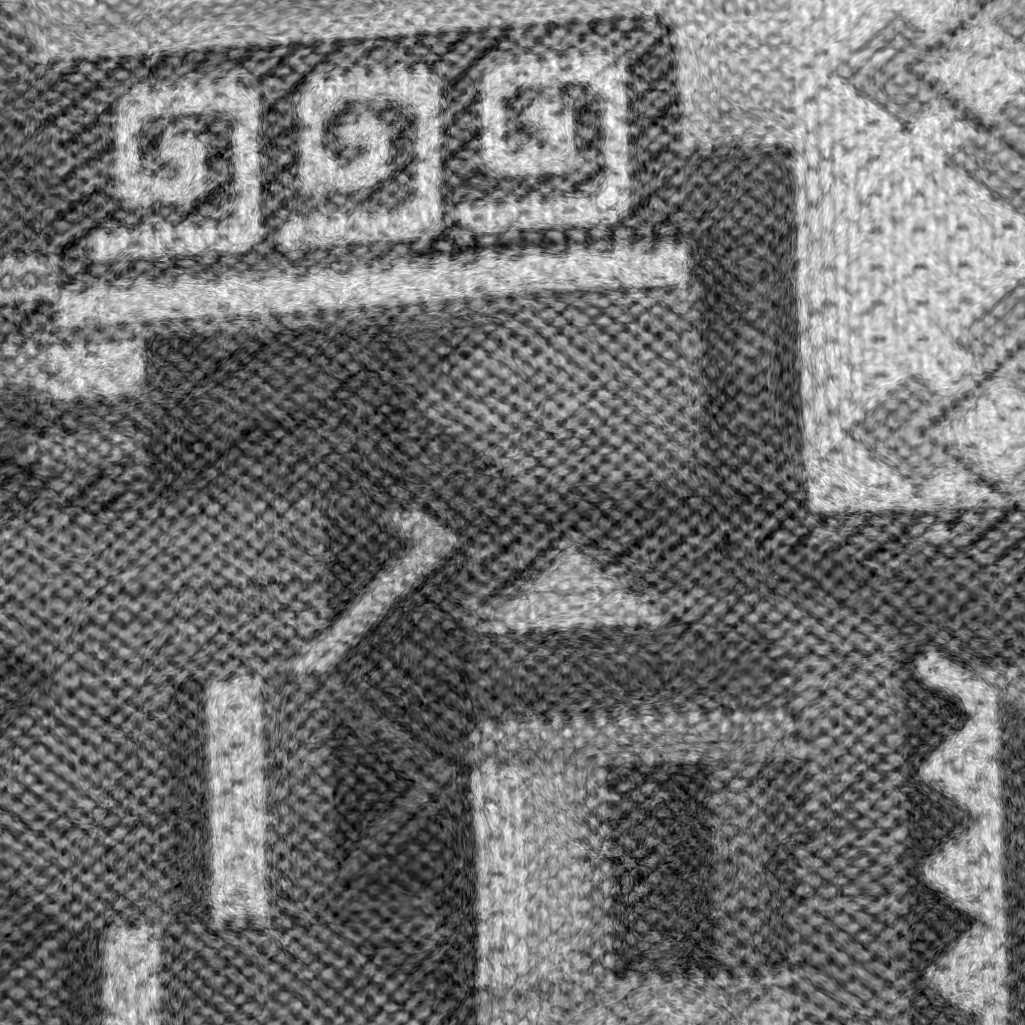
\includegraphics[width=\linewidth]{img/ch5/tex_zoom_in_stage_5.png}
\caption{}
\end{subfigure}
\begin{subfigure}{0.39\linewidth}
  \centering
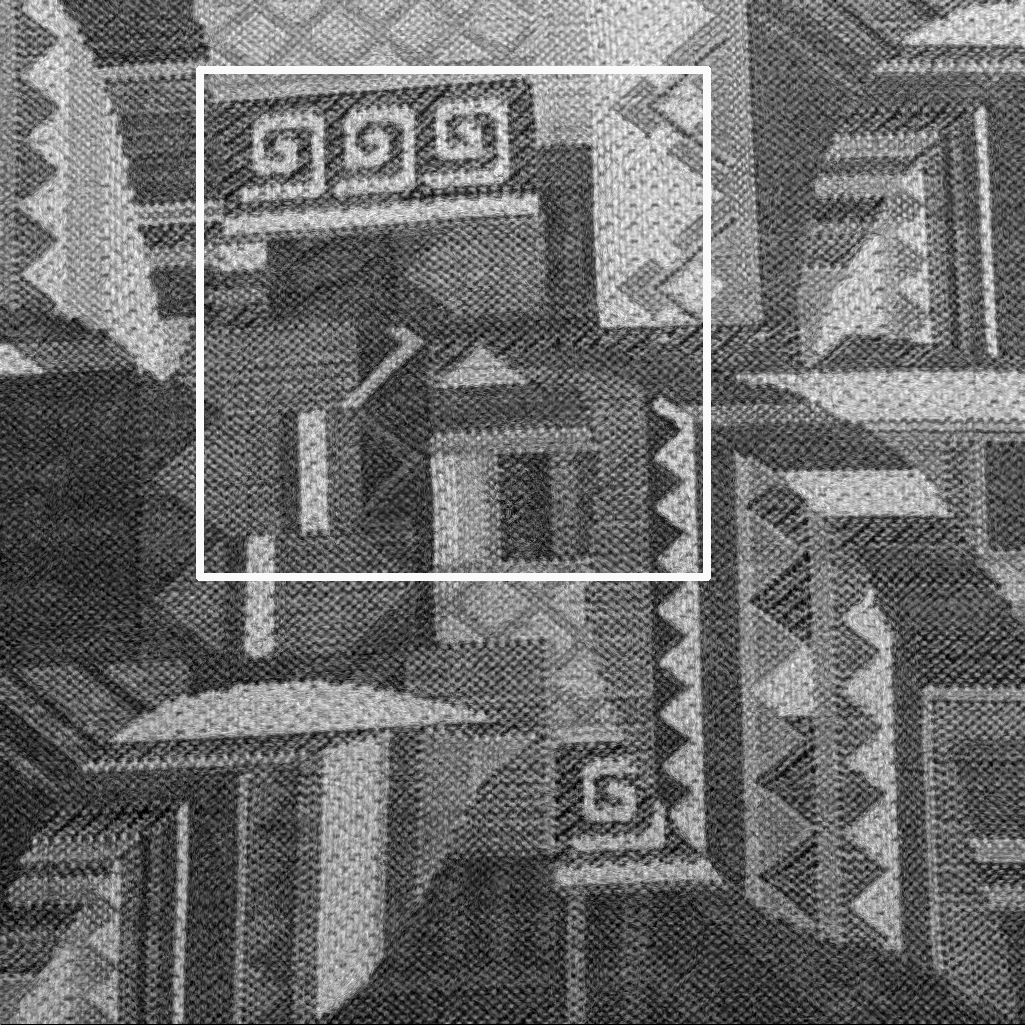
\includegraphics[width=\linewidth]{img/ch5/tex_stage_5.png}
\caption{}
\end{subfigure}
\begin{subfigure}{.19\linewidth}
  \centering
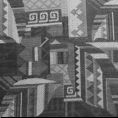
\includegraphics[width=\linewidth]{img/ch5/tex_zoom_out_stage_3.png}\\
\vspace{0.05cm}
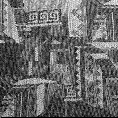
\includegraphics[width=\linewidth]{img/ch5/tex_zoom_out_stage_5.png}
\caption{}
\end{subfigure}
\caption{Woven Fabric Texture: (a) zoom in; (b) original image resolution; (c) zoom out.}
\label{f:pattern}
\end{figure}


The zoom-in is a detail with a resolution of $562\times 562$. marked by the white rectangle in Fig.~\ref{f:pattern}(b) and scaled up to $1025\times 1025$. Thus a zoom-in factor of $1.8$ times. It can be seen that the enlargement extrapolates the fine details of the image at this higher resolution beyond the original image. 

The zoom-out is a reduction of the entire image to $118\times 118$ pixels (shown enlarged to $501\times 501$ in the image for better viewing). The top sub-image is the network reconstruction at the appropriate level of detail (approximately 0.92). The bottom sub-image is point-sample nearest neighbor reduction. It can be seen that our reconstruction is a proper anti-aliased rendition of the image, while the sampled reduction exhibits aliasing artifacts.

These two behaviors in the experiment are manifestations of ``magnification'' and ``minification'', classical resampling regimes for respectively scaling up and down the image~\cite{pixel}. In the first case, it is necessary to interpolate the pixel values, and in the second case, it is required to integrate pixel values corresponding to the reconstructed pixel. The M-Net model accomplishes these tasks automatically.
Note that we have chosen a fractional scaling factors in both cases to demonstrate the continuous properties in space and scale of the M-Net~model.


\subsection{Anti-aliasing}

In the previous subsection we resorted to the level of detail control to guarantee an alias free rendering independently of the sampling resolution. However, this task was facilitated because we could use a constant level of detail for the entire image, due to the zooming in/out operation in 2D.

On the other hand, in texture mapping applications, this scenario is no longer the case. Typically, it requires to map a 2D texture onto a 3D surface that is rendered in perspective by a virtual camera. In such situation, the level of detail varies spatially depending on the distance of the 3D surface point from the camera. Here, proper anti-aliasing must compensate the foreshortening caused by a projective transformation. Next we present a simple example of anti-aliasing using the M-Net.

Let $I$ be a checkerboard image, $T$ be a \textit{homography} mapping the pixel coordinates $x=(x_1,x_2)$ of the screen to the texture coordinates $u=(u_1,u_2)$ of $I$, and $f:\R^2\times [0,N]\to \mathbb{R}$ be a M-net with $N$ stages approximating a multiresolution of $I$. 

\begin{figure}[!h]
\centering
% \includegraphics[width=0.48\linewidth]{img/ch5/alias-1.png}
% \includegraphics[width=0.48\linewidth]{img/ch5/alias-2.png}
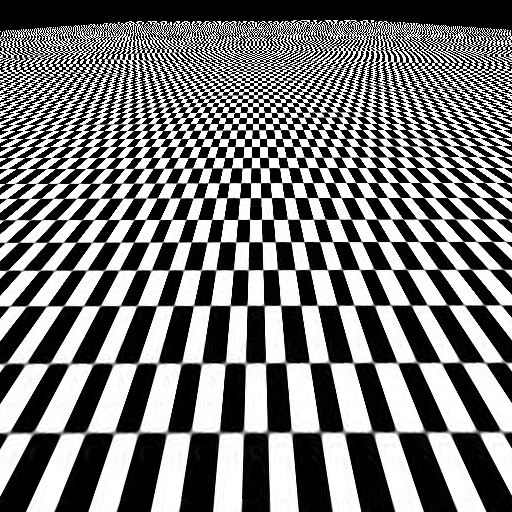
\includegraphics[width=0.46\linewidth]{img/ch5/im_0_alias.png}
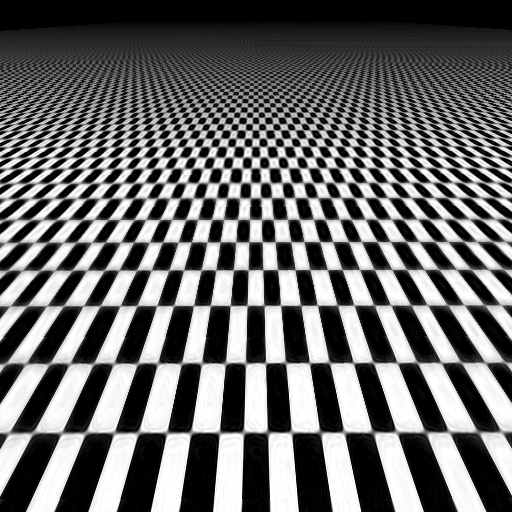
\includegraphics[width=0.46\linewidth]{img/ch5/im_0_anti_alias.png}
\centerline{(a)\hfil\hfil(b)}
\caption{Checkerboard in perspective: (a) point sampled texture rendition; (b) M-Net anti-aliased reconstruction.}
\label{f:alias}
\end{figure}

Fig~\ref{f:alias}(a) shows aliasing effects on the image $I$ after applying it to the inverse of $T$. We avoid such a problem using the multiresolution given by $f$. The result is presented in Fig~\ref{f:alias}(b). 

The above procedure reduces aliasing at large distances. Specifically,
we define the scale parameter $\lambda(x)$ for $f$ at a pixel $x$ using the Heckbert 's formula~\cite{heckbert1983texture}:

\begin{align*}
    \lambda(x)=\max\left\{\sqrt{\left(\frac{\partial u_1}{\partial x_1}\right)^2+\left(\frac{\partial u_2}{\partial x_1}\right)^2}, \sqrt{\left(\frac{\partial u_1}{\partial x_2}\right)^2+\left(\frac{\partial u_2}{\partial x_2}\right)^2}\right\}.
\end{align*}

Thus $\lambda(x)$ is the bigger length of the parallelogram generated by the vectors $\frac{\partial T}{\partial x_1}$ and $\frac{\partial T}{\partial x_2}$. 
We scale $\lambda$ such that $\lambda\big([-1,1]^2\big)\subset[0,N]$.
Thus, $f(x,\lambda(x))$ is the desired level of detail $\lambda(x)$ of $f$.

% \begin{figure}[!h]
% \centering
% 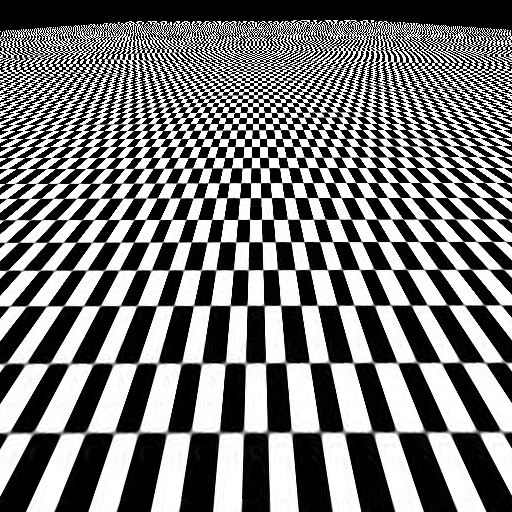
\includegraphics[width=0.48\linewidth]{img/ch5/im_0_alias.png}
% 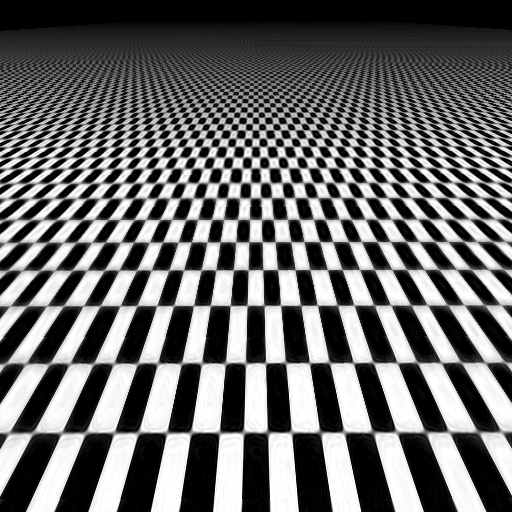
\includegraphics[width=0.48\linewidth]{img/ch5/im_0_anti_alias.png}
% 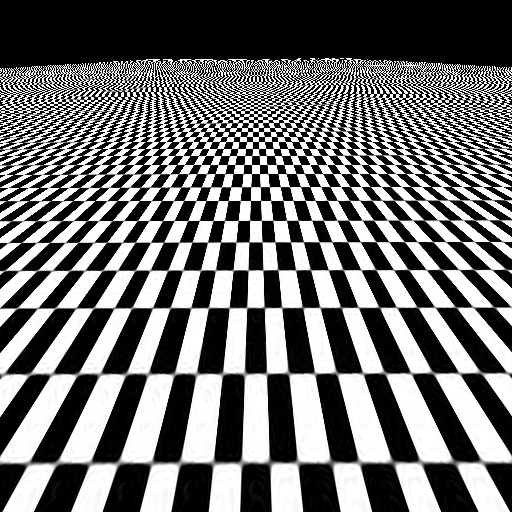
\includegraphics[width=0.48\linewidth]{img/ch5/im_1_alias.png}
% 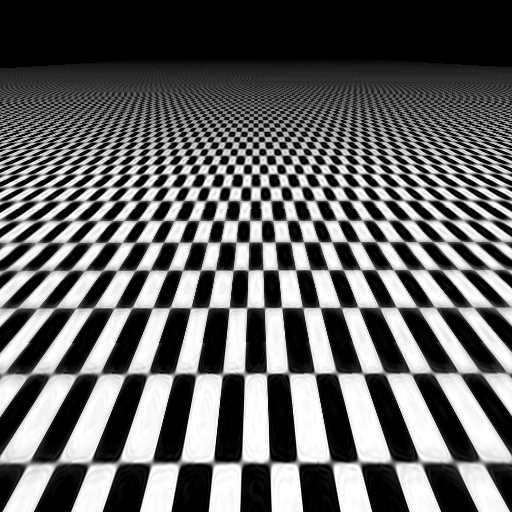
\includegraphics[width=0.48\linewidth]{img/ch5/im_1_anti_alias.png}
% \centerline{(a)\hfil\hfil(b)}
% \caption{Checkerboard in perspective: (a) point sampled texture rendition; (b) M-Net anti-aliased reconstruction.}
% \label{f:alias}
% \end{figure}


\section{Comparisons}

%In this section we show the comparison of the M-Net model with SIREN and BACON.
%
%We use as test data the image "Lena" with resolution of 513x513 pixels. Below we list the configuration of the three networks and results for the experiment.
%
%For the comparisons we adopted the same parameters of the M-Net model, as follows: Hidden Features = 96; Number of Levels = 7 (trained with Gaussian Pyramid);  w0 range =  [16, 112]; Model Size = 121824. 
%
%The PSNR of Reconstruction = 78 db.

In this section we compare the performance of MR-Net image representation with Siren~\cite{sitzmann2019siren} and Bacon~\cite{bacon2021}. 

First, we evaluate the quality of the original image fitting and the size of the representation for an instance of each model. Then, for MR-Net and BACON, the multiresolution models, we also evaluate the frequency spectra of the reconstructions in different scales. Finally, we proceed to a broader quantitative evaluation of the image reconstruction using the "Kodak Lossless True Color Image Suite" \cite{KodakDataset}, for which we compute the average Peak Signal to Noise Ratio (PSNR), the model size and the average running time for some different configurations of each model. 

\subsection{Image Fitting Evaluation}

We evaluate the capability of each model in the image fitting task using the ``Cameraman'' image, comparing the model size, given by the number of parameters of the model, and the reconstruction quality. We remark that to establish a fair comparison with SIREN we evaluate only the PSNR of the final full resolution image, which is $512\times 512$. Table~\ref{t:comp} summarizes the results.

\begin{table}[!h]
\centering
\small
\begin{tabular}{|l|r|r|r|}
\hline
Model & \# Params $(\downarrow)$ & PSNR $(\uparrow)$ & \# Levels \\
\hline
SIREN~\cite{sitzmann2019siren} & 198K & {\bf 34.1} dB & 1  \\
BACON~\cite{bacon2021} & 398K & 33.1 dB & 7 \\
MR-Net (Ours) & {\bf 196K} & 33.8 dB & 7  \\
\hline
\end{tabular}
\vspace{-0.1cm}
\caption{\label{tab:comp} Comparison with SIREN and BACON.}
\label{t:comp}
\end{table}

The M-Net parameters are: 1 hidden layer per stage; 96 hidden features per layer in the first 6 stages, and 256 hidden features in the last stage; $\omega \in [4, 256]$ and trained with a Gaussian Pyramid of 7 levels. The model size has 195648 parameters and the PSNR of the final image reconstruction is 33.8~dB. The model was trained for 300 epochs per stage.

For SIREN we employed the configuration of the image experiments and code released by the authors. The network parameters are: 3 hidden layers, 256 hidden features and $\omega_0$ equal to 30. The model size has $198400$ parameters and it has only 1 level of detail. The PSNR of the reconstructed image is 34.1 dB after training for 2000 epochs. Fig~\ref{f:siren} shows a comparison between our M-Net and SIREN. Notice that, although M-Net presents a PSNR close to Siren's in this example, visually, it seems that it can better represent high frequency details.

\begin{figure}[!h]
\centering
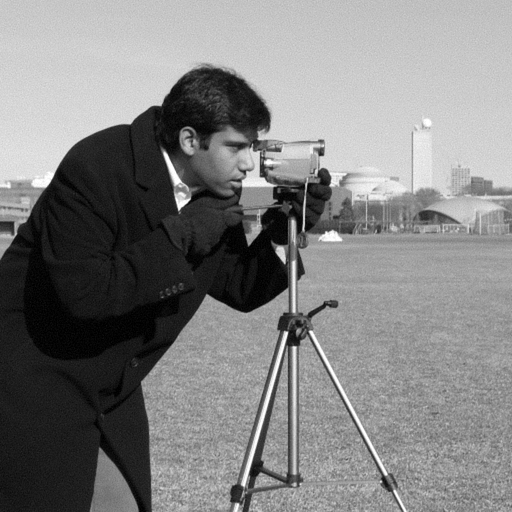
\includegraphics[width=0.44\linewidth]{img/ch5/rec-MR-Net.png}
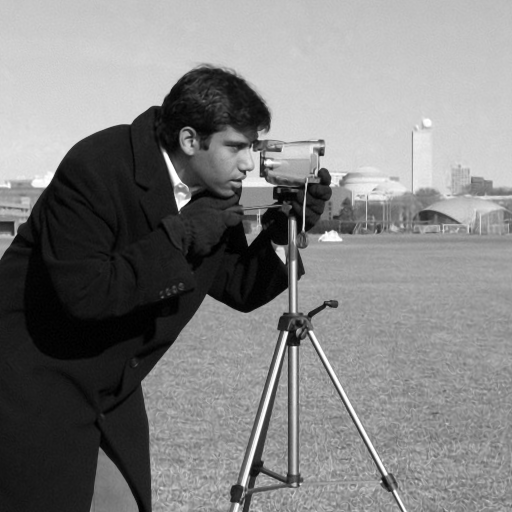
\includegraphics[width=0.44\linewidth]{img/ch5/rec-SIREN.png} \\
\centerline{M-Net \hfil SIREN}
\caption{Comparison of reconstructed images.}
\label{f:siren}
\end{figure}


For BACON we also based the configuration on their paper examples and code released by the authors, keeping 256 hidden features. However, we adjusted the number of hidden layers to 6 for it to output 7 levels of details as the M-Net in this setting. Accordingly, the total number of parameters is 398343. The PSNR of the original image level is 33.1 db.

Based on the experiments we conclude that MR-Net compared favorably in relation to BACON and SIREN, both in terms of representation size and quality of image reconstruction. The M-Net model is less than 50\% of the size of BACON model, while our reconstruction of the final image presents a comparable (slightly higher) PSNR. Compared to SIREN, the M-Net is about the same size in number of parameters, but it encodes 7 levels of details in a single network, in contrast with 1 level for SIREN. Additionally, the PSNR of both models are comparable, and M-Net looks sharper.

\subsection{Frequency Spectra Evaluation}
\label{sub:spectra-eval}

Figures~\ref{f:bacon} and~\ref{f:mnet} show the reconstructions and the frequency spectra for three levels of detail in the BACON and M-Net models respectively (1, 2, 6) and (3, 5, 7). Note that, as Bacon is not trained with multiresolution data, we select these levels to better match the frequency spectra between the representations.

\begin{figure}[!h]
\centering
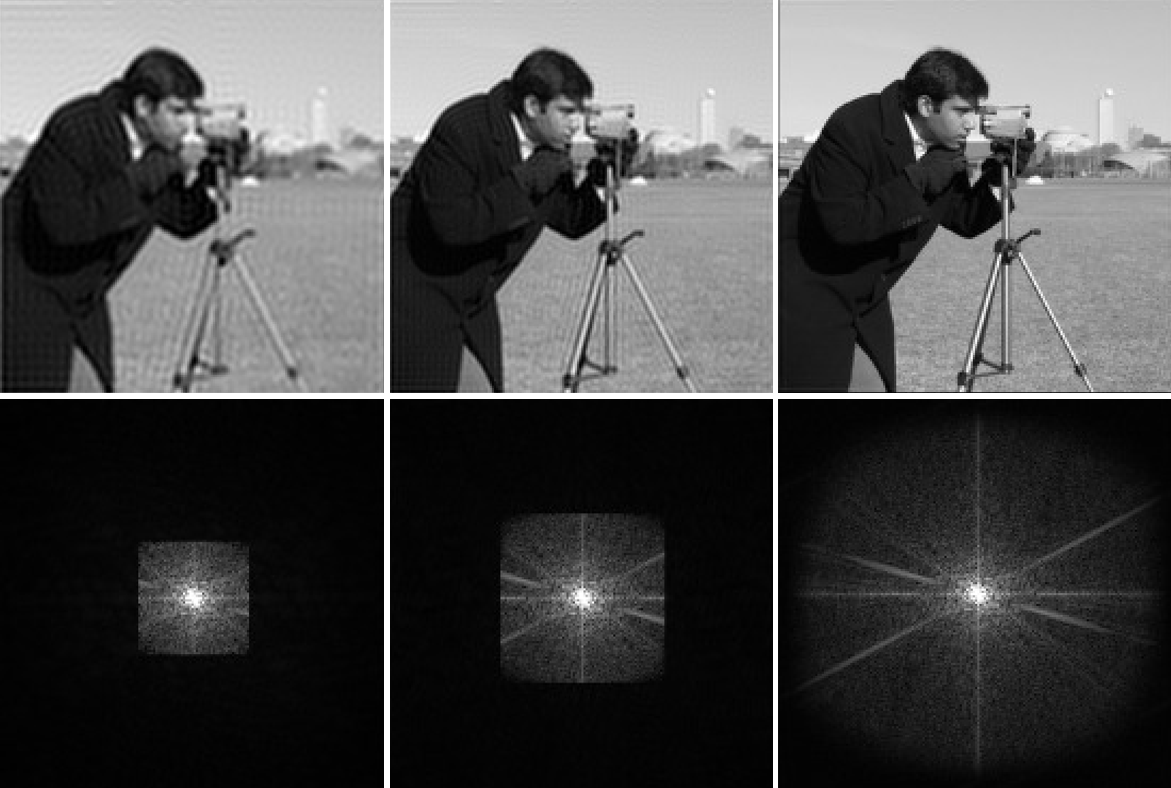
\includegraphics[width=0.85\linewidth]{img/ch5/bacon-3.png}
\centerline{\small Level 1 \hfil Level 2 \hfil Level 6}
\caption{BACON image reconstruction and frequency spectra.}
\label{f:bacon}
\end{figure}

\begin{figure}[!h]
\centering
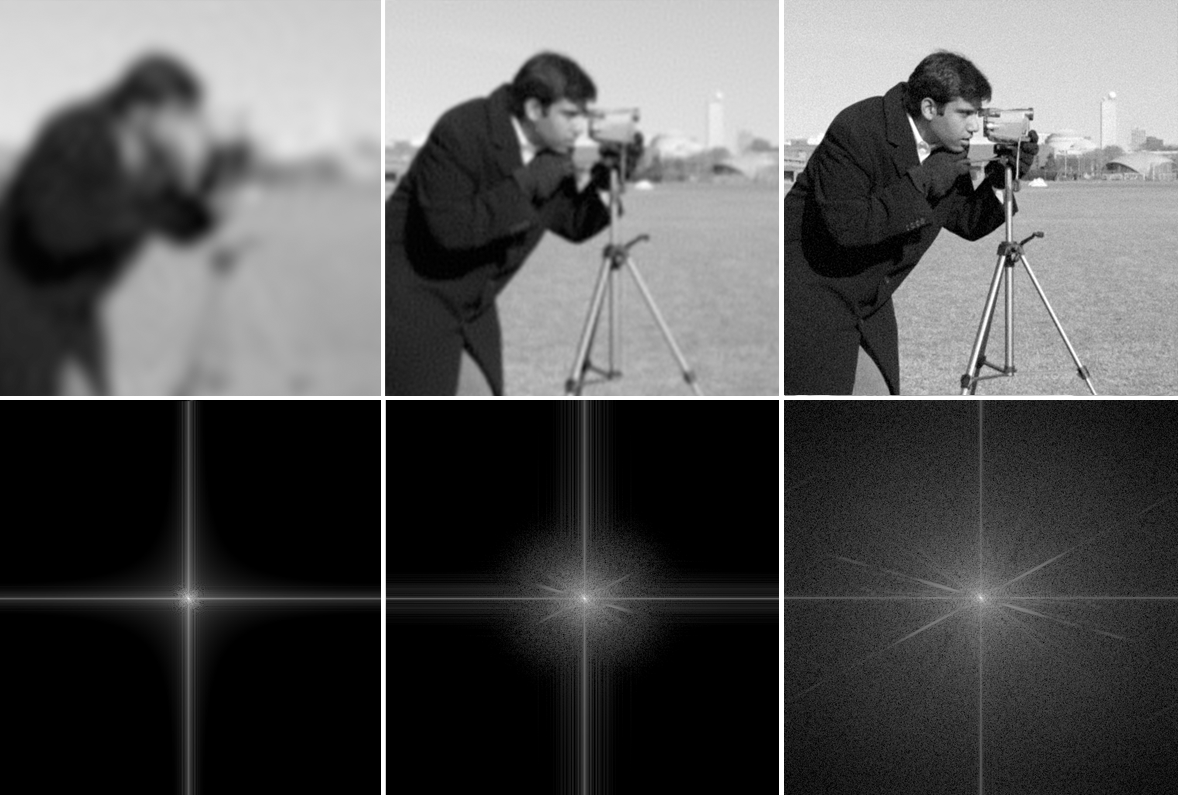
\includegraphics[width=0.85\linewidth]{img/ch5/m-net-3.png}
\centerline{\small Level 3 \hfil Level 5 \hfil Level 7}
\caption{M-Net image reconstruction and frequency spectra.}
\label{f:mnet}
\end{figure}


BACON controls the frequency band for Level of Detail by truncating the spectrum. Fig~\ref{f:bacon} shows that the center of the spectrum images of Levels 1, 2, 6 are all similar. This is analogous to applying a low-pass filter with non-ideal shape in the frequency domain, which results in an image with ringing effect (see the silhouettes propagating all over Fig~\ref{f:bacon} (left)). M-Net does not present such artifacts. Fig~\ref{f:mnet} resembles more faithfully what would be expected to be the process of sequentially applying Gaussian filters in a high-resolution image.

\subsection{Kodak Dataset Evaluation}\label{sub:kodak}

The ``Kodak Lossless True Color Image Suite" is a set of 24 images, originally $768 \times 512$ in size, that were extensively used in the image processing literature. For each image, we center crop a square of $512\times 512$ pixels, convert it to grayscale and evaluate the PSNR, model size and training time using different network configurations of each model. The average results over this dataset are summarized in Table~\ref{t:kodak}. 

We present the training time in a relative scale. All models were trained in a NVidia GeForce RTX 3080 with 10GB of GPU memory. The longest average running time observed was 40 minutes and 33 seconds (2433 seconds) when training an instance of BACON with 6 hidden layers and 256 neurons per layer (Bacon\_6hl\_256). Therefore, we display this row as 100\% and all others as a fraction of it.


\begin{table}[!h]
\centering
\small
\begin{tabular}{|l|r|r|r|}
\hline
Model                    & \# Params $(\downarrow)$ & PSNR $(\uparrow)$ & Time $(\downarrow)$ \\
\hline
SIREN$_\text{3hl\_256hf}$        & 198K      & 41.93    & 8.7\%       \\
SIREN$_\text{4hl\_256hf}$        & 264K      & 44.63    & 11.0\%      \\
SIREN$_\text{5hl\_256hf}$        & 330K      & 46.25    & 13.6\%      \\
SIREN$_\text{3hl\_512hf}$        & 790K      & 48.57    & 23.8\%      \\
\hline
BACON$_\text{5hl\_128hf}$        & 84K       & 27.42    & 36.2\%      \\
BACON$_\text{6hl\_128hf}$        & 101K      & 28.23    & 44.1\%      \\
BACON$_\text{4hl\_256hf}$        & 266K      & 33.69    & 60.8\%      \\
BACON$_\text{5hl\_256hf}$        & 332K      & 34.13    & 75.7\%      \\
BACON$_\text{6hl\_256hf}$        & 398K      & 34.31    & 100.0\%     \\
\hline
% MNet$_\text{5hl\_96hf}$          & 85K       & XXXX    & 5.4\%       \\
% MNet$_\text{6hl\_96hf}$          & 104K      & XXXX    & 6.7\%       \\
% MNet$_\text{7hl\_96hf}$          & 123K      & XXXX    & XXX\%       \\
MNetCap$_\text{2stg\_256hf}$    & 117K      & 35.14    & 3.4\%       \\
MNet$_\text{7stg\_24\_256hf}$          & 193K      & 38.42    & 9.3\%       \\
MNet$_\text{7stg\_96\_256hf}$          & 196K      & 35.04    & 9.6\%       \\
MNet$_\text{6stg\_24\_288hf}$          & 197K      & 40.85    & 8.2\%       \\
MNetCap$_\text{128\_192\_256}$ & 195K      & 41.05    & 8.0\%       \\
MNetCap$_\text{3stg\_256hf}$           & 332K      & 45.46    & 11.4\%     \\
\hline
\end{tabular}
\vspace{-0.1cm}
\caption{\label{tab:kodak} Comparisons on Kodak Lossless True Color Image Suite. We present the training time relative to BACON$_\text{6hl\_256hf}$ which took 2433 seconds to train.}
\label{t:kodak}
\end{table}


We evaluate 4 SIREN instances: respectively 3, 4 and 5 hidden layers with 256 neurons per layer; and 3 hidden layers with 512 neurons per layer. For Bacon, we evaluate 5 instances: 5 and 6 hidden layers with 128 neurons per layer; and 4, 5, and 6 hidden layers with 256 neurons per layer. 

All M-Net stages have depth $2$, so we vary the number of stages and their width. As we are only evaluating the  reconstruction at the final level, we trained M-Net with and without multiresolution data. Notice that we have more flexibility on the M-Net configuration as each MR-Module can have a different size. We decided to explore a few configurations with heterogeneous stages, choosing smaller modules for the coarsest levels, and bigger modules for the finest ones.

When training with a Gaussian pyramid, we evaluate MNet$_\text{7stg\_96\_256hf}$ with 7 stages and width in [96, 96, 96, 96, 96, 96, 256]; MNet$_\text{7stg\_24\_256hf}$ with 7 stages and width in [24, 32, 64, 96, 96, 160, 256]; and MNet$_\text{6stg\_24\_288hf}$ with 6 stages and width in [24, 32, 64, 96, 160, 288]. Although very different, these models have about the same number of total parameters. When training capacity based instances using only the original image, we evaluate MNetCap$_\text{2stg\_256hf}$  with 2 stages and width $256$; MNetCap$_\text{3stg\_256hf}$ with 3 stages and width $256$; and MNetCap$_\text{128\_192\_256}$ with 3 stages and width $128$, $192$, and $256$ in each respective~stage.

In general, inside each model category, as we increase the total number of parameters, the quality of the reconstruction also increases. Moreover, SIREN and M-Net models of the same size present a comparable performance in terms of PSNR, while BACON achieves lower values at the level of the original image. The exception occurs when we compare the M-Net models MNet$_\text{7stg\_24\_256hf}$ and MNet$_\text{7stg\_96\_256hf}$. Both models have 7 stages of multiresolution, but while the latter has a homogeneous architecture on all but the last level, the former distributes its capacity allocating less parameters in the initial levels. We think this heterogeneous distribution is better because on the coarsest levels we have lower frequencies and a less detailed signal to fit. When comparing MNet$_\text{7stg\_24\_256hf}$ and MNet$_\text{6stg\_24\_256hf}$, we see that as we remove one stage, and increase the width of the finest stages to keep a comparable model size, the performance of the model also increases. 

Each M-Net model is trained for 2000 epochs per stage, while the others are trained for 5000 epochs. Although we train M-Net for more epochs, notice that due to our scheduled training scheme, we only update the parameters of a single stage each 2000 epochs. Besides that, when training with multiresolution data, the coarsest stages are trained with fewer samples. This way M-Net trains faster than the other models even when the number of parameters is bigger and the number of epochs too. 

Training a 6 stages M-Net with 197182 parameters (MNet$_\text{6stg\_24\_288hf}$) for 12000 epochs takes a similar amount of time (199 seconds) as training a SIREN with 3 hidden layers and 198401 parameters for 5000 epochs (211 seconds); and both are faster than training a BACON model with fewer parameters (BACON$_\text{5hl\_128hf}$ takes 881 seconds). The highest quality M-Net model in this evaluation, a M-Net capacity based with 331523 parameters and 3 levels of details (MNetCap$_\text{3stg\_256hf}$), trained for 6000 epochs takes 278 seconds, which is only 15\% of the time to train a BACON model of the same size (Bacon$_\text{5hl\_256hf}$ takes 1842 seconds) and is comparable to training a 20\% smaller SIREN for 5000 epochs (Siren$_\text{4hl\_256hf}$ takes 267 seconds).


\section{Considerations for Other MR-Net subclasses}\label{sec:considerations}

Until now, we have only used the M-Net subclass. In this section, we briefly present a comparison of M-Net with the others MR-Net subclasses.

For S-Net, we define a configuration composed of 3 stages, with 1000, 2000, and 4000 hidden features per layer respectively, which add to a total of 28000 parameters. For the L-Net, the configuration follows 3 stages with 2 hidden layers with 40, 60, and 80 neurons for each layer. This L-Net version has an overall number of parameters of 24.280. For the last variant, the M-Net, we set 3 stages with 1 hidden layer each. Each stage has 30, 40, and 80 hidden features per layer respectively where the final number of parameters was 23.100. During training the S-Net, L-Net, and M-Net were trained at the maximum of 4000, 2000, and 2000 epochs respectively and we test 10 different images with resolution $128 \times 128$ for training. 
As we can see in Table \ref{t:comp-variants}, on average, considering the PSNR, the M-Net outperforms the other variants when reconstructing images.

\begin{table}[!h]
\centering
\small
\begin{tabular}{|l|r|r|r|}
\hline
Model & \# Params $(\downarrow)$ & PSNR $(\uparrow)$  \\
\hline
S-Net & 28000 & 42.1 dB  \\
L-Net & 24280 & 47.8 dB \\
M-Net & {\bf 23100} & {\bf 51.1} dB   \\
\hline
\end{tabular}
\vspace{-0.3cm}
\caption{\label{tab:comp-variants} Comparison between the MR-Net Variants.}
\label{t:comp_variantes}
\end{table}

Nonetheless, here it is appropriate to make a few considerations about the S-Net and L-Net variants.

The S-Net represents the image as a weighted sum of sine functions. In that sense, S-Net is equivalent to BACON and other Multiplicative Filter Networks based on sinusoidal atoms. As such, it is amenable to represent periodic visual patterns. Figure \ref{f:albert-snet} presents the gradient magnitude and frequency spectra from an image predicted by S-net, where it has three stages.

\begin{figure}[!h]
\centering
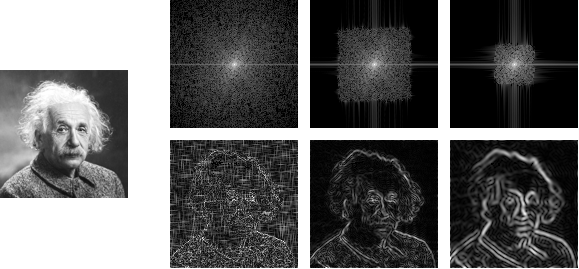
\includegraphics[width=0.9\linewidth]{img/ch5/albert.png}
\caption{S-Net Gradient Magnitude and frequency spectra.}
\label{f:albert-snet}
\end{figure}


The L-Net image representation comprises a sum of level-of-detail stages given by independent MR-Modules. The relation of this representation with the Laplacian Pyramid makes it suitable for image operations in the gradient domain. Figure \ref{f:albert-lnet} shows the L-Net reconstruction for the same image as S-Net and the frequency spectra for both L-Net stages. 

\begin{figure}[!h]
\centering
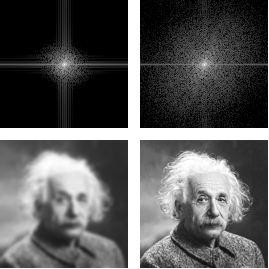
\includegraphics[width=0.98\linewidth]{img/ch5/albert-lnet.png}
\caption{L-Net reconstruction and frequency spectra.}
\label{f:albert-lnet}
\end{figure}



%TO DO REWRITE EXPERIMENTS S-NET, L-NET, M-NET

%We intend to study and compare the three variants of the MR-Net architecture and also to develop imaging applications in dir,ections pointed out above for L-Net, complementing the ones we have presented in the paper for M-Net.

\section{Limitations}

In this section we present an assessment of our results, as well as, its limitations, and a discussion of future directions for our research.

We found that choosing appropriate values for the $\omega$ parameter, which defines the spatial frequency of the network first layer, is important to achieve proper results. 
When using a shallow sinusoidal network such as the S-Net, we can use the Nyquist frequency as a direct reference to pick the frequency intervals at each stage. However, a deep sinusoidal network such as the M-Net can learn higher frequencies that were not present in the initialization. 

In our experiments, we have determined the $\omega$ values for initialization of the frequency bands empirically, testing values below the Nyquist frequency as described in Sec \ref{s-frequency-initialization}. To better harness the power of sinusoidal neural networks, it is important to develop mathematical theories to understand how the composition of sine functions introduces new frequencies based on the initialization of the network. In future works we intend to investigate the use of the results in \cite{novello2022understanding} to compute or bound these~frequencies.